\documentclass[border=2pt]{standalone}

%Drawing
\usepackage{tikz}
\tikzset{>=latex}

% Notation
\usepackage{amsmath}

\begin{document}
	
	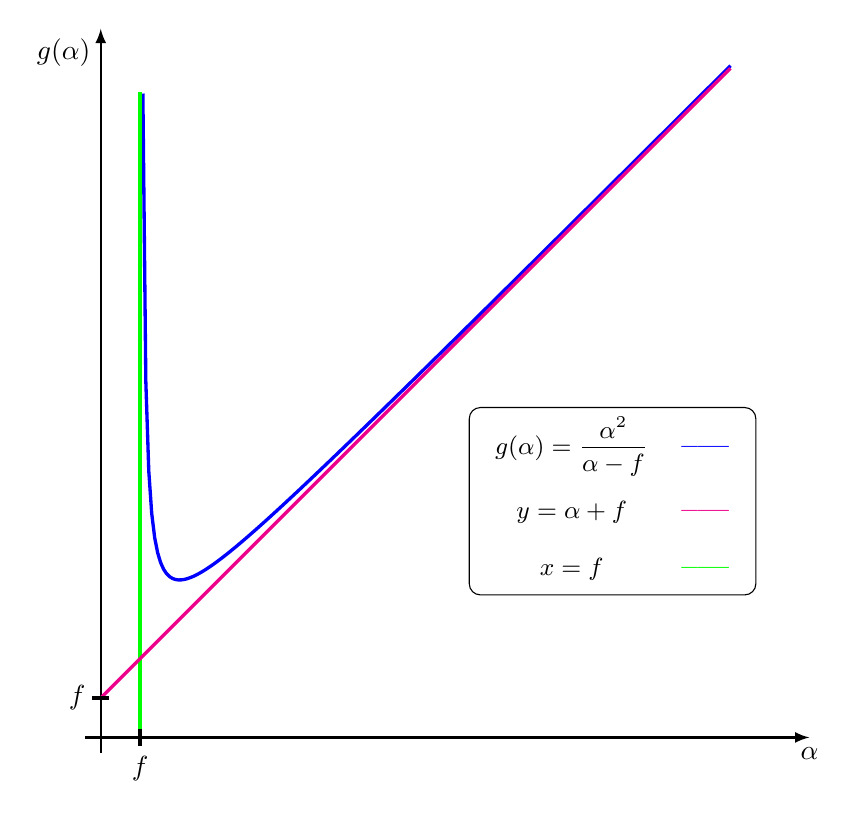
\begin{tikzpicture}
		% Grid
%		\draw[help lines] (-1,-1) grid (10,10);

		% Axis
		\draw[->, thick] (-0.2,0) -- (9,0) node[below] {$\alpha$}; 
		\draw[->, thick] (0,-0.2) -- (0,9) node[below left] {$g(\alpha)$};
		
		% Graphs
		\draw[very thick, blue, domain=0.535:8, samples=200] plot (\x,{\x^2/(\x-0.5)});
		\draw[very thick, green, domain=0:8.2, samples=200] plot (0.5,\x);
		\draw[very thick, magenta, domain=0:8, samples=200] plot (\x,{\x+0.5});
		
		% Values on Axis		
		\draw[very thick] (0.5, -3pt) -- (0.5, 3pt); 
		\node at (0.5, -0.4) {$f$};
		%	
		\draw[very thick] (-3pt, 0.5) -- (3pt, 0.5); 
		\node at (-0.3, 0.5) {$f$};
		
		% Table with Infos on the Right Corner
		\node[rounded corners, draw] at (6.5,3) {%
			\begin{tabular}{c c}
				\small$g(\alpha) = \dfrac{\alpha^2}{\alpha - f}$ & \color{blue}\textbf{–––} \\[4mm] 
				\small$y = \alpha + f$ & \color{magenta}\textbf{–––} \\[3mm] 
				\small$ x = f $ & \color{green}\textbf{–––}
			\end{tabular}};
	\end{tikzpicture}
	
\end{document}
